\section{想定利用環境}

% 利用場所・空間的条件
本システムは，オフィスや研究室など，複数のユーザが同一空間で作業を行う環境での利用を想定している．
同一空間に滞在している状況では，特定の人間関係や事前の約束に依存せず，偶発的に帰宅を共にする可能性が生じやすい．
本システムは，図\ref{fig:monitor}に示すように，部屋の滞在者全体に向けて帰宅に関する情報を発信するため，共用空間内にモバイルディスプレイを設置した．
一般に，執務空間や研究室において，部屋全体から常時視認可能な表示位置を確保するのは構造的に難しい場合が多い．
本システムではこのような実環境上の制約を前提とした上で，滞在者の視界に入りやすい位置への設置により空間全体に向けた情報共有が成立する構成を採用している．
\begin{figure}[htb]
  \centering
  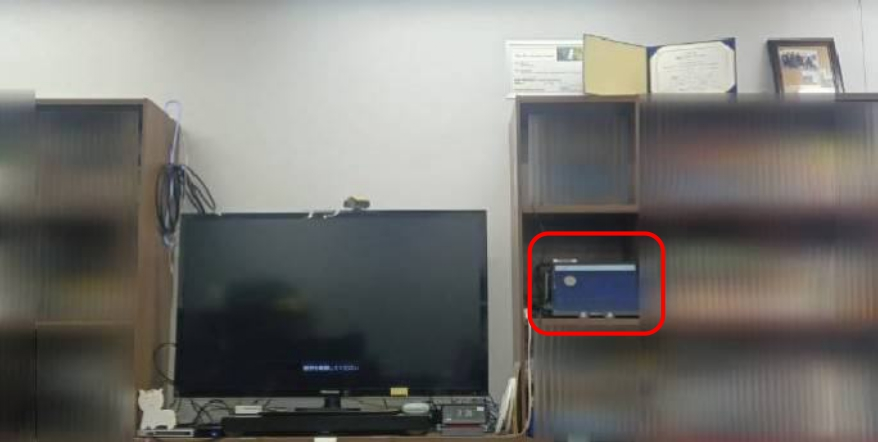
\includegraphics[width=0.8\linewidth]{fig/monitor.jpg} % suzuki
  \caption{モバイルディスプレイの設置例}
  \label{fig:monitor}

\end{figure}


% このように空間全体に向けての情報の提示により，個別の関係性に基づく誘いかけを必要としない設計としている．
% これにより，本システムの利用は任意であり，ユーザは自身の判断で帰宅同行に参加できる．
% また，参加しない選択を行った場合でも周囲に違和感を与えにくいよう配慮している．

% 想定ユーザ
また，業務終了時刻や帰宅時刻が厳密に固定されておらず，帰宅時刻をある程度調整可能なユーザが存在する環境を想定する．
一方で，帰宅時刻が組織的な規定や運用によって一律に定められ，ユーザに対して実質的な拘束力を持つ環境は，本システムの対象とはしない．
このような環境では，個々のユーザが帰宅時刻を調整する余地が小さく，本システムによるアプローチが成立しにくい．
また，特定の同行相手に行動が固定されやすく，他の滞在者との交流促進につながりにくいと考えられるためである．

% 前提条件
他にも，実際の滞在履歴に基づき帰宅予測時刻を取得するため，過去の滞在履歴が継続的に蓄積できる環境である必要がある．
滞在履歴の取得手法自体は限定せず，個人単位で識別可能な入退室ログなどの既存の仕組みを利用できるとともに，何らかの手段によって現在の滞在者をある程度リアルタイムに把握できる設備を前提とする．
また，帰宅予測時刻は，3章で述べた先行研究で提案された外部システム\cite{hayashi}により算出・提供されるものを利用する．


必須条件ではないが，Web APIなどで公共交通機関の時刻表を取得できると，時刻表情報を別途構築・管理する必要がなく，システムの導入や運用の負担を軽減できるためより望ましい．
公共交通機関の時刻表情報については，国や自治体が公開するGTFS形式のオープンデータや，事業者・外部サービスが提供する経路探索APIを通じて取得できる事例が既に存在する\cite{opendata}\cite{navi}\cite{eki}.
公共交通機関の時刻表情報を外部から取得する仕組み自体は現在広く普及しており，今後も同様のデータ提供形態が継続的に更新・提供されると考えられる．
このように，本研究で想定する公共交通機関の時刻表取得は，特殊な前提を必要とするものではなく，既存のAPIやオープンデータの活用により実現可能である．